\documentclass{article}

% Language Setting
\usepackage[english]{babel}

% Set page size and margins
\usepackage[letterpaper,top=2cm,bottom=2cm,left=3cm,right=3cm,marginparwidth=1.75cm]{geometry}

% Useful packages
\usepackage{amsmath}
\usepackage{graphicx}
\usepackage{listings}
\usepackage[colorlinks=true, allcolors=blue]{hyperref}

\title{Question 29: Cardboard Box Problem}
\author{Alec Him}
\date{}

\begin{document}
\maketitle


\section{Introduction}
This document contains the mathematical derivation and calculations for solving the cardboard box problem. The goal is to maximize the volume of the cardboard box formed by cutting 4 squares of \( x\) length on each corner and given area \( A \).
\begin{figure}[h!]
    \centering
    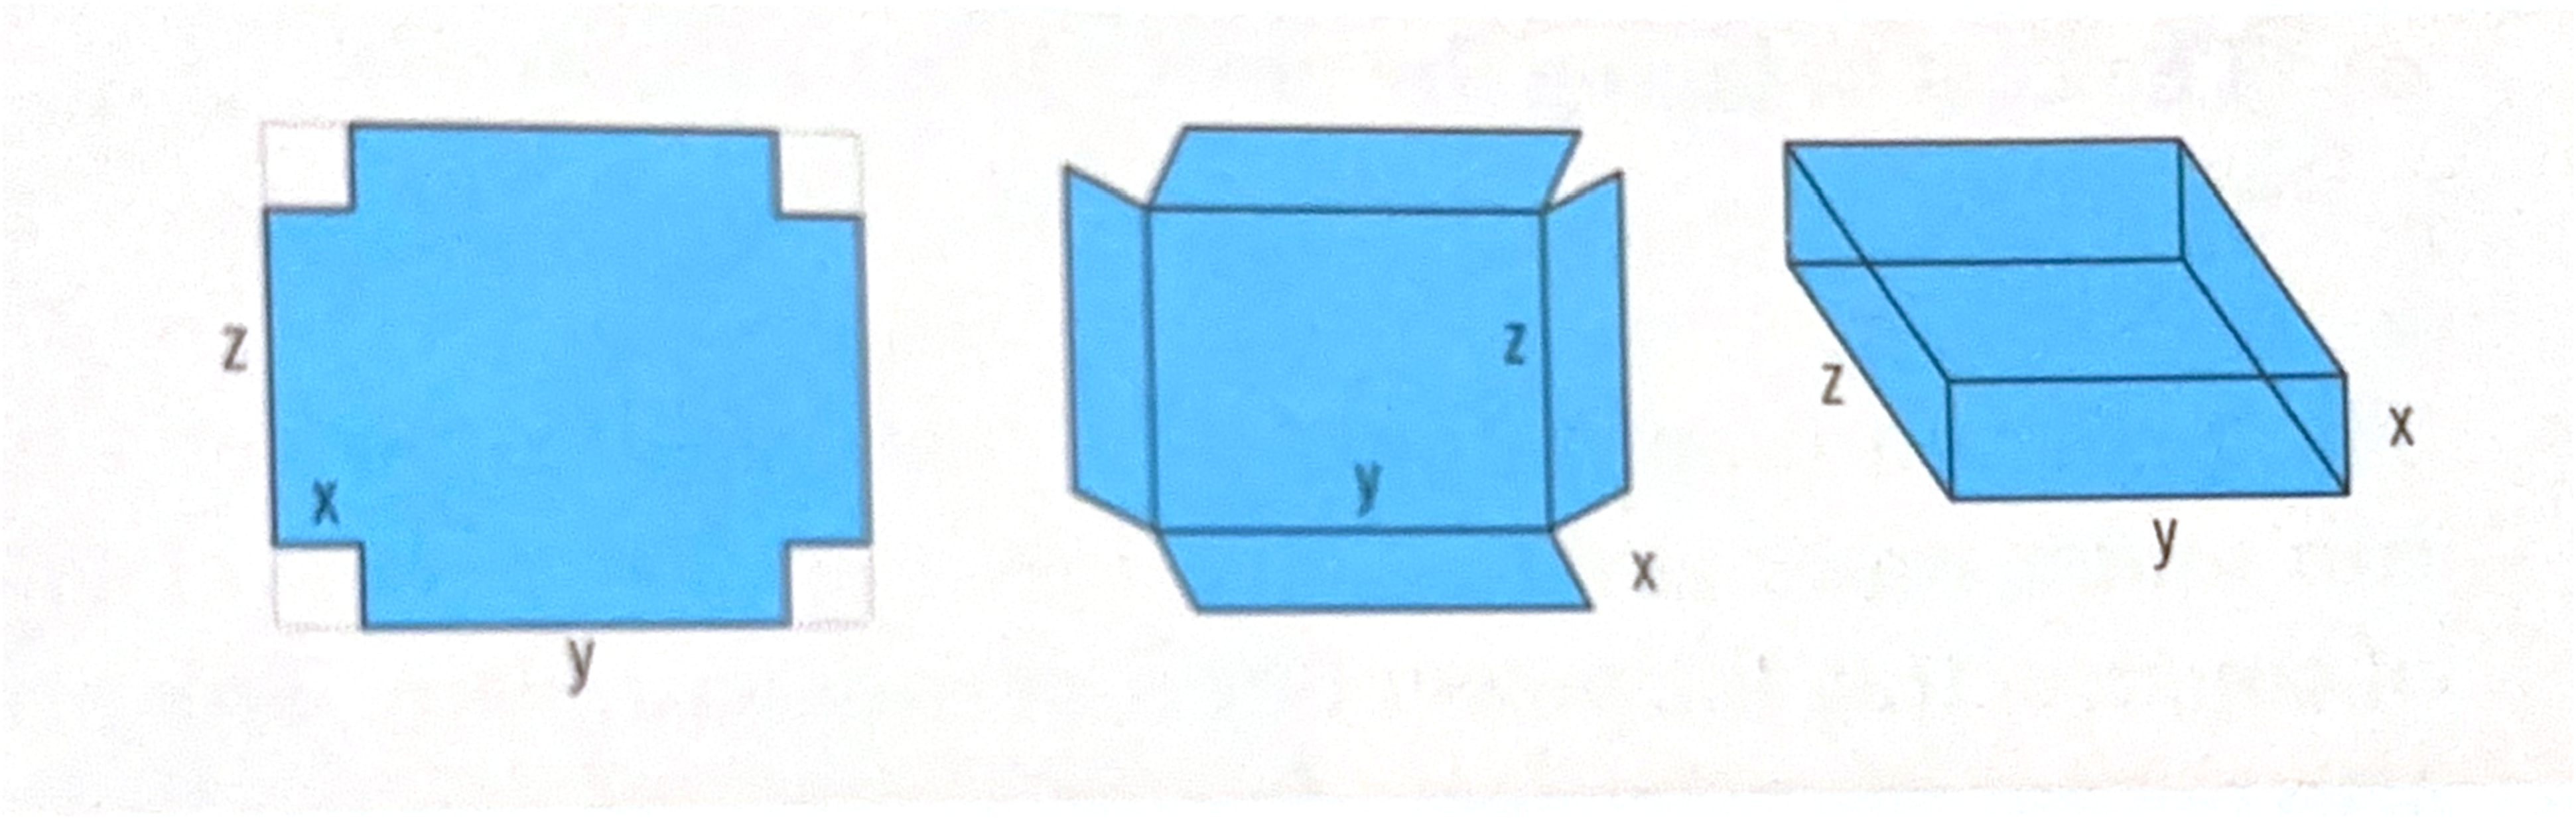
\includegraphics[width=0.6\textwidth]{Figure1.pdf}
    \caption{Diagram of the cardboard box problem showing 3 figures where we cut a square of \( x \) size of a cardboard box with a width \(z \) and length \( y \).}
    \label{fig.Graph}
\end{figure}

\section{Variables}
\begin{itemize}
    \item \( A \) : Area of the flat cardboard (user inputted as \texttt{area}).
    \item \( l \) : Length of the flat cardboard.
    \item \( w \) : Width of the flat cardboard.
    \item \( x \) : Side of the square being cut from the cardboard.
    \item \( y \) : Length of the cardboard box.
    \item \( z \) : Width of the cardboard box.
    \item \( h \) : Height of the cardboard box, which is equal to \( x \) (since the size of the square determines the height of the box).
\end{itemize}


\section{Formulation and Derivation}
The area of the flat cardboard is given by:
\begin{equation}
    A = l \cdot w
\end{equation}
To find \( l \) and \( w \):
\begin{equation}
    l = \frac{A}{w}, \quad w = \frac{A}{l}
\end{equation}
The new dimensions after cutting squares of side \( x \) are:
\begin{equation}
    y = l - 2x, \quad z = w - 2x
\end{equation}
The volume of the resulting box is:
\begin{equation}
    V = y \cdot z \cdot x
\end{equation}
Expanding:
\begin{align*}
    V &= (l - 2x)(w - 2x)(x) \\
      &= lwx - 2lx^2 - 2wx^2 + 4x^3 \\
      &= Ax - 2lx^2 - 2wx^2 + 4x^3
\end{align*}


\section{Maximization using Calculus}
To maximize \( V \), differentiate \( V \) with respect to \( x \) and set \(\frac{dV}{dX} = 0\).
\begin{align}
    \frac{dV}{dx} = V' = \frac{d}{dx}\left[4x^3 - 2lx^2 - 2wx^2 + Ax\right] = 0 \\
    V' = 12x^2 - 4lx - 4wx + A = 0
\end{align}
Solving for \( x \) using the quadratic formula:
\begin{equation}
    x = \frac{-\left(-4l - 4w\right) \pm \sqrt{\left(-4l - 4w\right)^2 - 4\left(12\right)\left(A\right)}}{2\left(12\right)}
\end{equation}
Simplifying:
\begin{equation}
    \label{eq:quadratic}
    x = \frac{4l + 4w \pm \sqrt{16l^2 + 16w^2 - 48A}}{24}
\end{equation}
However, this approach requires knowing \( l \) and \( w \) in advance, which is not possible without additional constraints (e.g., a given aspect ratio). Testing in code revealed that in many cases, the maximum volume could not be determined correctly.


\section{Revised Iterative Approach}
Since \( l \) and \( w \) must satisfy \( A = l \cdot w \), we iterate over factored pairs of \( A \), checking each valid configuration. For every divisor \( i \) of \( A \), there exists a corresponding divisor \( \frac{A}{i} \). We only check up to \( \sqrt{A} \), reducing complexity to \( O(\sqrt{A}) \).

For each factor pair, we iterate over possible \( x \) values to maximize \( V \). The additional iteration over \( x \) increases complexity beyond \( O(\sqrt{A}) \), making it dependent on the step size and range of \( x \). If iterating over a range \( R \) with step size \( s \), the additional cost is roughly \( O(R/s) \), leading to an overall complexity of approximately:
\begin{equation}
    O(\sqrt{A} \cdot R/s)
\end{equation}
This adds overhead but ensures a more precise maximum volume calculation.

\section{Conclusion}
The calculus approach failed due to the unknown ratio of \( l \) and \( w \). The revised iterative method, though slightly more complex, guarantees an accurate solution by considering all factorable pairs of \( A \) and iterating over possible values of \( x \). While the additional loop increases runtime, the tradeoff ensures correctness.

\end{document}
